% コンパイル（slide/20261107/ で実行。PDFは slide/out/20261107/ 、他は build/）:
%   ../lualatex-dated.sh -synctex=1 -interaction=nonstopmode -file-line-error -output-directory=out survey_kawamotostyle_20261107_handout_v2.tex
\documentclass[aspectratio=169,10pt,t,handout]{beamer}
\usepackage[ja]{labslide}
\usepackage{multirow}
% 本文・見出し・脚注など、指定されている文字サイズを一律に 1pt 大きくする．
\makeatletter
\newdimen\labvtwo@size
\newskip\labvtwo@skip
\let\labvtwo@set@fontsize\set@fontsize
\def\set@fontsize#1#2#3{%
  \@defaultunits\labvtwo@size#2pt\relax\@nnil
  \advance\labvtwo@size by 1pt\relax
  \@defaultunits\labvtwo@skip#3pt\relax\@nnil
  \advance\labvtwo@skip by 1pt\relax
  \begingroup
    \edef\x{\endgroup
      \noexpand\labvtwo@set@fontsize{\unexpanded{#1}}{\strip@pt\labvtwo@size}{\the\labvtwo@skip}%
    }\x
}
\makeatother
\usetikzlibrary{fit,backgrounds,calc,positioning}

\makeatletter
\setlength{\beamer@frametopskip}{0mm}
\makeatother
\setbeamertemplate{frametitle}{%
  \vspace{4.2mm}%
  {\usebeamerfont{frametitle}\color{ink}\insertframetitle\par}%
  \vspace{0.4mm}%
  {\color{ruleblue}\rule{\textwidth}{0.7pt}\par}%
  \vspace{1.1mm}%
  \ifx\insertframesubtitle\@empty\else
    {\footnotesize\color{muted}\insertframesubtitle\par}%
    \vspace{1.2mm}%
  \fi
}

\definecolor{cviolet}{HTML}{F3E8F6}
\definecolor{cviolettt}{HTML}{7A458E}
\definecolor{cred}{HTML}{F8E6E6}
\definecolor{credtt}{HTML}{C44545}
\renewcommand{\usecardcolor}[1]{%
  \def\cardfill{cgreen}%
  \def\cardtitlec{cgreentt}%
  \ifstrequal{#1}{red}{%
    \def\cardfill{cred}%
    \def\cardtitlec{credtt}%
  }{}%
  \ifstrequal{#1}{orange}{%
    \def\cardfill{corange}%
    \def\cardtitlec{corangett}%
  }{}%
  \ifstrequal{#1}{blue}{%
    \def\cardfill{cblue}%
    \def\cardtitlec{cbluett}%
  }{}%
  \ifstrequal{#1}{green}{%
    \def\cardfill{cgreen}%
    \def\cardtitlec{cgreentt}%
  }{}%
  \ifstrequal{#1}{violet}{%
    \def\cardfill{cviolet}%
    \def\cardtitlec{cviolettt}%
  }{}%
  \ifstrequal{#1}{plain}{%
    \def\cardfill{cplain}%
    \def\cardtitlec{cplaintt}%
  }{}%
  \ifstrequal{#1}{gray}{%
    \def\cardfill{cplain}%
    \def\cardtitlec{cplaintt}%
  }{}%
}

\graphicspath{{fig/}{../20261007/fig/survey/}}

\kicker{サーベイ}
\title{安全保障と好み選択を\\両立する局所プランナ}
\subtitle{CATNAV と SEA-Nav}
\date{2026年11月}

\newcommand{\li}{%
  \ifvmode\else\par\fi
  \noindent\hangindent=1.15em\hangafter=1
  \makebox[1.15em][l]{\textcolor{ruleblue}{\textbullet}}\ignorespaces}
\newcommand{\lii}{%
  \ifvmode\else\par\fi
  \noindent\hspace{1.0em}\hangindent=2.15em\hangafter=1
  \makebox[1.05em][l]{\textcolor{muted}{\textendash}}\ignorespaces}

\newcommand{\cardbalance}{\par\vspace*{-\topskip}\vspace{0pt plus 1fill}}
\newcommand{\takeawaybalance}[1]{%
  \par\vspace{0.15em plus 1fill}%
  \begingroup
  \setlength{\fboxsep}{5pt}%
  \noindent\colorbox{ink}{%
    \parbox[c]{\dimexpr\textwidth-10pt\relax}{%
      \color{white}\footnotesize #1}}%
  \endgroup
}

\RenewDocumentCommand{\infocard}{O{green} o m m}{%
  \usecardcolor{#1}%
  \IfValueTF{#2}{\def\cardminh{#2}}{\def\cardminh{0pt}}%
  \begin{tikzpicture}[baseline=(card.north)]
    \node[
      anchor=north west,
      fill=\cardfill,
      text width=\dimexpr\linewidth-14pt\relax,
      minimum height=\cardminh,
      inner xsep=6.5pt,
      inner ysep=4pt,
      align=flush left
    ] (card) {%
      {\color{\cardtitlec}\bfseries #3}\par\vspace{0.15em}%
      {\color{body}\footnotesize #4\par}%
    };
  \end{tikzpicture}%
}

\begin{document}

\begin{frame}[plain]
  \labtitlepage{}
\end{frame}

% ハンドアウト v3 の p2 をそのまま使う（調査スライドの制御系に対応）
\begin{frame}{研究テーマ ｜ ロボットの制御系}
  \centering
  \begin{tikzpicture}[node distance=6.5mm]
    \node[kworange, text width=24mm, minimum height=8mm] (c) {コントローラ};
    \node[kwgreen, text width=24mm, minimum height=8mm, right=of c] (p) {局所プランナ};
    \node[kwblue, text width=24mm, minimum height=8mm, right=of p] (g) {歩行モデル};
    \node[kwpurple, text width=24mm, minimum height=8mm, right=of g] (m) {モータ};
    \draw[kwarr] (c) -- (p)
      node[midway, below=4mm, font=\scriptsize, text=muted] {目標座標};
    \draw[kwarr] (p) -- (g)
      node[midway, below=4mm, font=\scriptsize, text=muted] {目標速度};
    \draw[kwarr] (g) -- (m)
      node[midway, below=4mm, font=\scriptsize, text=muted] {トルク};
  \end{tikzpicture}

  \vspace{1.5em}
  \includegraphics[width=\textwidth,height=35mm,keepaspectratio]{img001.png}

  \takeaway{一般的に、入力は3つの変換を経てモータに届く}
\end{frame}

% ハンドアウト v3 の p3 をそのまま使う（調査スライドの安全保障と好み選択に対応）
\begin{frame}{研究テーマ ｜ 局所プランナ}
  \centering
  \begin{tikzpicture}[node distance=6.5mm]
    \node[kworange, text width=24mm, minimum height=8mm, opacity=0.2] (c) {コントローラ};
    \node[kwgreen, text width=24mm, minimum height=8mm, right=of c] (p) {局所プランナ};
    \node[kwblue, text width=24mm, minimum height=8mm, right=of p] (g) {歩行モデル};
    \node[kwpurple, text width=24mm, minimum height=8mm, right=of g, opacity=0.2] (m) {モータ};
    \draw[kwarr] (c) -- (p)
      node[midway, below=4mm, font=\scriptsize, text=muted] {目標座標};
    \draw[kwarr] (p) -- (g)
      node[midway, below=4mm, font=\scriptsize, text=muted] {目標速度};
    \draw[kwarr] (g) -- (m)
      node[midway, below=4mm, font=\scriptsize, text=muted] {トルク};
  \end{tikzpicture}

  \includegraphics[width=\textwidth,height=35mm,keepaspectratio]{img002.png}

  \takeaway{目標速度を、「安全保障」と「好み選択」の両方に対応させる局所プランナの研究を行う}
\end{frame}

\begin{frame}{好みと安全に関する論文}
  \infocard[green][24mm]{好み ｜ CATNAV}{%
    \li Cached Vision-Language Traversability for Efficient Zero-Shot Robot Navigation
    \li Potnis et al.，arXiv，2026
    \li VLM で意味的なリスクを見積もり，複数経路から好みの経路を選ぶ}
  \vspace{0.4em}
  \infocard[blue][24mm]{安全 ｜ SEA-Nav}{%
    \li Efficient Policy Learning for Safe and Agile Quadruped Navigation in Cluttered Environments
    \li Chen et al.，arXiv，2026
    \li 微分可能な安全フィルタを方策の中に入れ，密集環境を短時間で学ぶ}

  \takeaway{1本目は好みを経路選択で表し，2本目は安全を速度指令の制約で表す．}
\end{frame}

% ---------- CATNAV ----------

\begin{frame}{CATNAV}
  \source{Potnis et al., arXiv, 2026, Fig.~1}
  \centering
  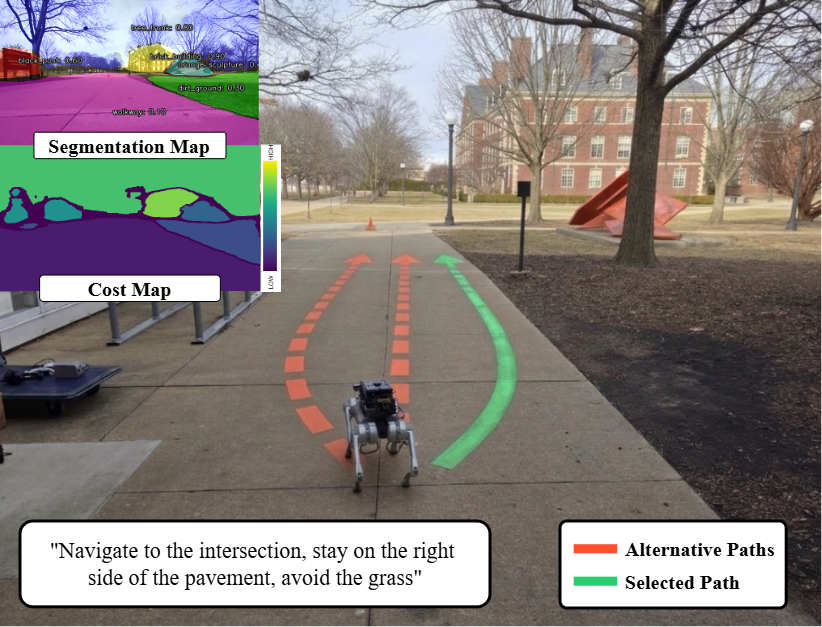
\includegraphics[height=48mm]{catnav_teaser.png}

  \takeaway{CLIP-Seg で領域を分け，コストマップを作り，候補経路から一本を選ぶ．二段階で好みを選ぶ．}
\end{frame}

\begin{frame}{背景}
  \source{Potnis et al., arXiv, 2026}
  \infocard[orange][22mm]{走破リスク}{%
    \li ロボットの物理的な能力に対して評価する必要がある
    \li 屋外は動的障害物と地形への配慮
    \li 屋内は人や壊れやすいものへの配慮}
  \vspace{0.35em}
  \begin{columns}[T,onlytextwidth]
    \begin{column}{0.32\textwidth}
      \infocard[plain][24mm]{学習ベース}{%
        \li 大量の学習データが要る
        \li 分布外に弱い}
    \end{column}
    \hfill
    \begin{column}{0.32\textwidth}
      \infocard[blue][24mm]{VLM}{%
        \li コスト化すると柔軟な推論を捨てやすい
        \li 毎回問うと計算が重い}
    \end{column}
    \hfill
    \begin{column}{0.32\textwidth}
      \infocard[orange][24mm]{VLA}{%
        \li 速度を直接出せる
        \li なぜその道かを人が読みにくい}
    \end{column}
  \end{columns}

  \takeaway{少ないデータと計算で，数値と人間らしい判断の両方を残したい．}
\end{frame}

\begin{frame}{課題}
  \source{Potnis et al., arXiv, 2026}
  \cardbalance
  \infocard[blue][14mm]{1}{\li 少ないアノテーションでも，高い推論能力が欲しい}
  \vspace{0.28em}
  \infocard[orange][14mm]{2}{\li 少ない計算資源でも，高い周波数で動いてほしい}
  \vspace{0.28em}
  \infocard[green][14mm]{3}{\li 数値だけでなく，社会的で柔軟な判断をしてほしい}
  \takeawaybalance{できれば，その判断が人にとって解釈可能であってほしい．}
\end{frame}

\begin{frame}{貢献}
  \source{Potnis et al., arXiv, 2026}
  \cardbalance
  \infocard[blue][16mm]{貢献 1 ｜ ゼロショットのリスク}{%
    \li タスク固有の学習はせず，VLM の推論で意味的リスク値を推定する}
  \vspace{0.28em}
  \infocard[orange][16mm]{貢献 2 ｜ 評価の再利用}{%
    \li 画像特徴から類似シーンを見つけ，リスク評価をキャッシュして問い合わせを減らす}
  \vspace{0.28em}
  \infocard[green][16mm]{貢献 3 ｜ 経路の選択}{%
    \li RGB に乗せた複数経路から，視覚的に安全な経路を VLM に選ばせる}
  \takeawaybalance{VLM の柔軟な推論を残したまま，必要な問い合わせを減らす．}
\end{frame}

\begin{frame}{方法}
  \source{Potnis et al., arXiv, 2026, Fig.~2}
  \centering
  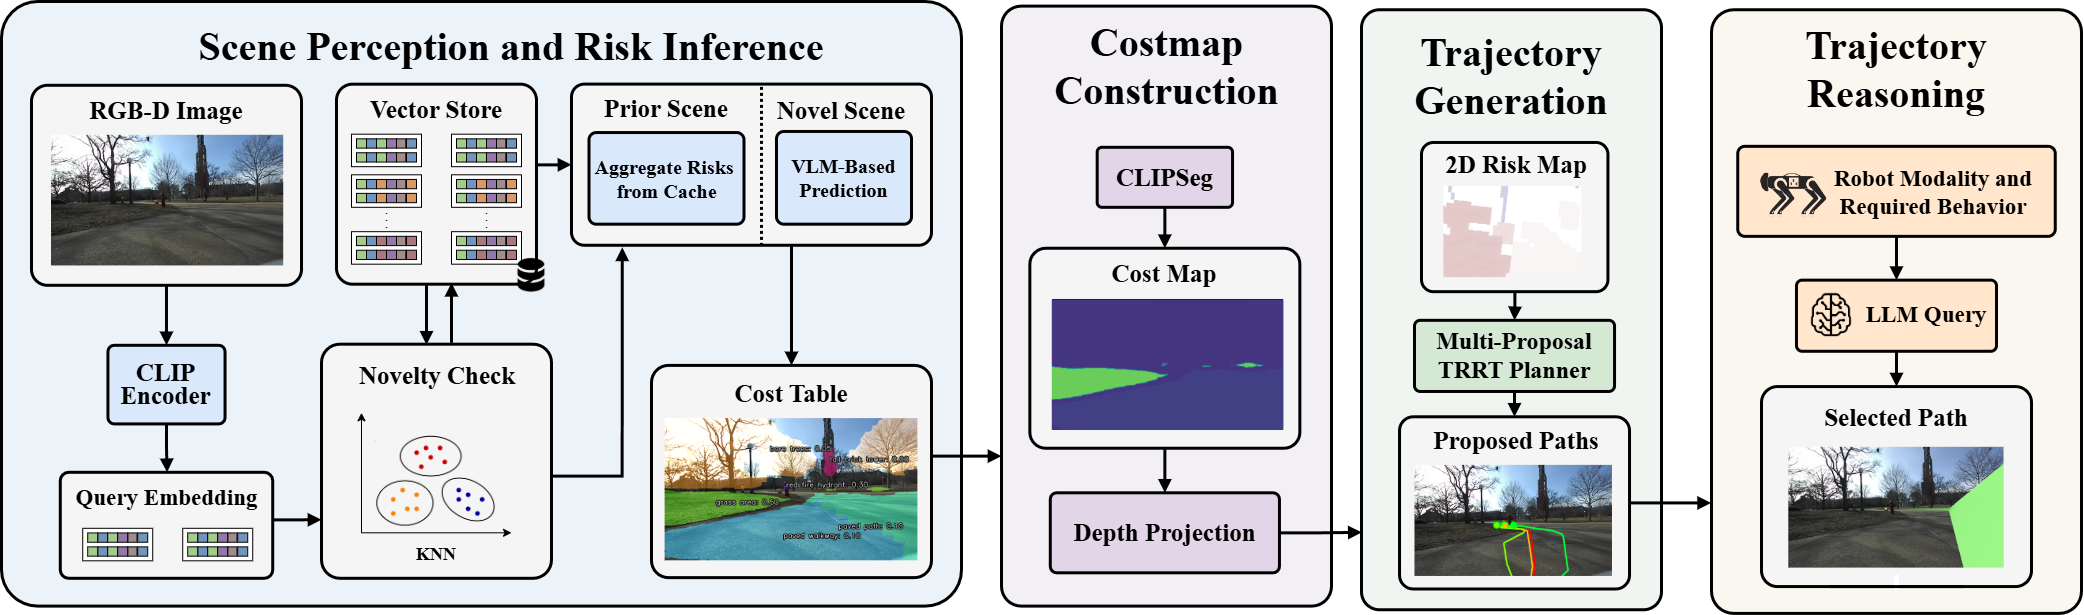
\includegraphics[width=\textwidth,height=46mm,keepaspectratio]{catnav_pipeline.png}

  \takeaway{認識，経路生成，経路選択の順で行動が決まる．}
\end{frame}

\begin{frame}{ゼロショット認識}
  \source{Potnis et al., arXiv, 2026}
  \centering
  \begin{tikzpicture}[
      font=\footnotesize,
      box/.style={align=center, minimum height=11mm, text width=34mm, inner sep=2pt}
    ]
    \node[kwblue, box] (clip) at (0,1.55) {CLIP Encoder\\{\scriptsize 画像特徴量}};
    \node[kworange, box] (vlm) at (5.6,1.55) {VLM\\{\scriptsize 物体検出とリスク推定}};
    \node[kwgreen, box, text width=28mm] (cache) at (2.8,0) {キャッシュ};
    \node[kwblue, box] (seg) at (0,-1.55) {CLIP-Seg\\{\scriptsize セグメンテーション}};
    \node[kwgreen, box] (map) at (5.6,-1.55) {コストマップ};
    \draw[kwarr] (clip.south) -- (cache.north west)
      node[midway, left, font=\scriptsize, text=muted] {画像特徴量};
    \draw[kwarr] (vlm.south) -- (cache.north east)
      node[midway, right, font=\scriptsize, text=muted] {コストテーブル};
    \draw[kwarr] (cache.south west) -- (seg.north)
      node[midway, left, font=\scriptsize, text=muted] {物体名ラベル};
    \draw[kwarr] (cache.south east) -- (map.north)
      node[midway, right, font=\scriptsize, text=muted] {リスク値};
  \end{tikzpicture}

  \takeaway{特徴量とコストテーブルはキャッシュに集まり，そこからマップを作る．}
\end{frame}

\begin{frame}{貢献 1 ｜ VLM によるリスク推定}
  \source{Potnis et al., arXiv, 2026}
  \begin{columns}[T,onlytextwidth]
    \begin{column}{0.48\textwidth}
      \infocard[orange][28mm]{聞く内容}{%
        \li 画像中の物体名と，そのリスクを出させる
        \li コストテーブルは $[\text{物体名},\,\text{リスク値}]$
        \li タスク用の学習データは使わない}
    \end{column}
    \hfill
    \begin{column}{0.48\textwidth}
      \infocard[blue][28mm]{いつ聞くか}{%
        \li 処理は重く，毎回だと遅延が出る
        \li シーンが新しいときだけ問い合わせる
        \li 人や構造物は高め，路面は低めになる}
    \end{column}
  \end{columns}

  \takeaway{VLM の知識だけでリスクを見積もれるが，毎回は処理したくない．}
\end{frame}

\begin{frame}{CLIP Encoder ｜ 画像特徴量}
  \source{Potnis et al., arXiv, 2026}
  \infocard[blue][16mm]{特徴量}{%
    \li CLIP Encoder で画像を 768 次元の特徴量ベクトルにする
    \li キャッシュ内の特徴量と比較する}
  \vspace{0.3em}
  \infocard[orange][18mm]{新規性の閾値}{%
    \li 閾値より特徴が違うときだけ，物体検出とリスク推定を実行する
    \li それ以外は，キャッシュ内の近傍 $k$ 件のリスク値を使う}
  \vspace{0.3em}
  \infocard[green][14mm]{再利用}{%
    \li 似たシーンでは VLM に聞かない．聞いた結果はキャッシュへ追加する}

  \takeaway{画像特徴が近いときは，過去のリスク評価をそのまま使う．}
\end{frame}

\begin{frame}{CLIP-Seg ｜ セグメンテーション}
  \source{Potnis et al., arXiv, 2026}
  \infocard[blue][20mm]{反応値}{%
    \li コストテーブルの物体名ラベルとの反応値を画素ごとに得る
    \li 最も反応が高い物体が，その画素に映っているとみなす
    \li 微小領域の数値は，バイリニア補間で画像サイズまで引き伸ばす}
  \vspace{0.35em}
  \infocard[green][16mm]{ゼロショット}{%
    \li 物体名へのアテンションの最大値で，学習なしに領域を分ける}

  \takeaway{物体名との反応の最大値で，ゼロショットにセグメンテーションする．}
\end{frame}

\begin{frame}{CLIP-Seg ｜ コストマップ}
  \source{Potnis et al., arXiv, 2026}
  \infocard[orange][18mm]{画素からコストへ}{%
    \li 各画素のクラスに，対応するリスク値を乗せてコストマップを作る
    \li 深度を使い，3D から 2D のコストマップへ落とす
    \li この 2D マップの上で経路を引く}
  \vspace{0.35em}
  \begin{columns}[T,onlytextwidth]
    \begin{column}{0.32\textwidth}
      \infocard[green][16mm]{低い}{\li 舗装など．例として $0.1$}
    \end{column}
    \hfill
    \begin{column}{0.32\textwidth}
      \infocard[orange][16mm]{中間}{\li 草など．例として $0.3$}
    \end{column}
    \hfill
    \begin{column}{0.32\textwidth}
      \infocard[red][16mm]{高い}{\li 人や構造物．例として $0.7$}
    \end{column}
  \end{columns}

  \takeaway{領域にコストを乗せ，3D から 2D に変換してマップとして使う．}
\end{frame}

\begin{frame}{軌道生成と軌道選択}
  \source{Potnis et al., arXiv, 2026, Fig.~2}
  \begin{columns}[T,onlytextwidth]
    \begin{column}{0.56\textwidth}
      \infocard[plain][10mm]{1．中央}{\li 遷移ベース RRT（T-RRT）で経路を作る}
      \vspace{0.16em}
      \infocard[blue][10mm]{2．左 ／ 3．右}{\li 安全条件の範囲で，最大 $d$ だけ左右へずらす}
      \vspace{0.16em}
      \infocard[orange][12mm]{4．リスク軌道}{\li 安全閾値を緩めた条件で，T-RRT をやり直す}
    \end{column}
    \hfill
    \begin{column}{0.40\textwidth}
      \centering
      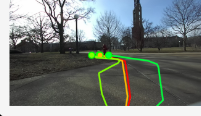
\includegraphics[width=\linewidth,height=28mm,keepaspectratio]{catnav_paths.png}\\[0.25em]
      {\scriptsize\color{muted} 赤が中央，緑が左右，黄がリスク軌道}
    \end{column}
  \end{columns}

  \takeaway{複数の軌道を作り，VLM に道の種類と安全な理由を考えて選ばせる．}
\end{frame}

\begin{frame}{結果 ｜ VLM によるコスト評価}
  \source{Potnis et al., arXiv, 2026, Fig.~5}
  \centering
  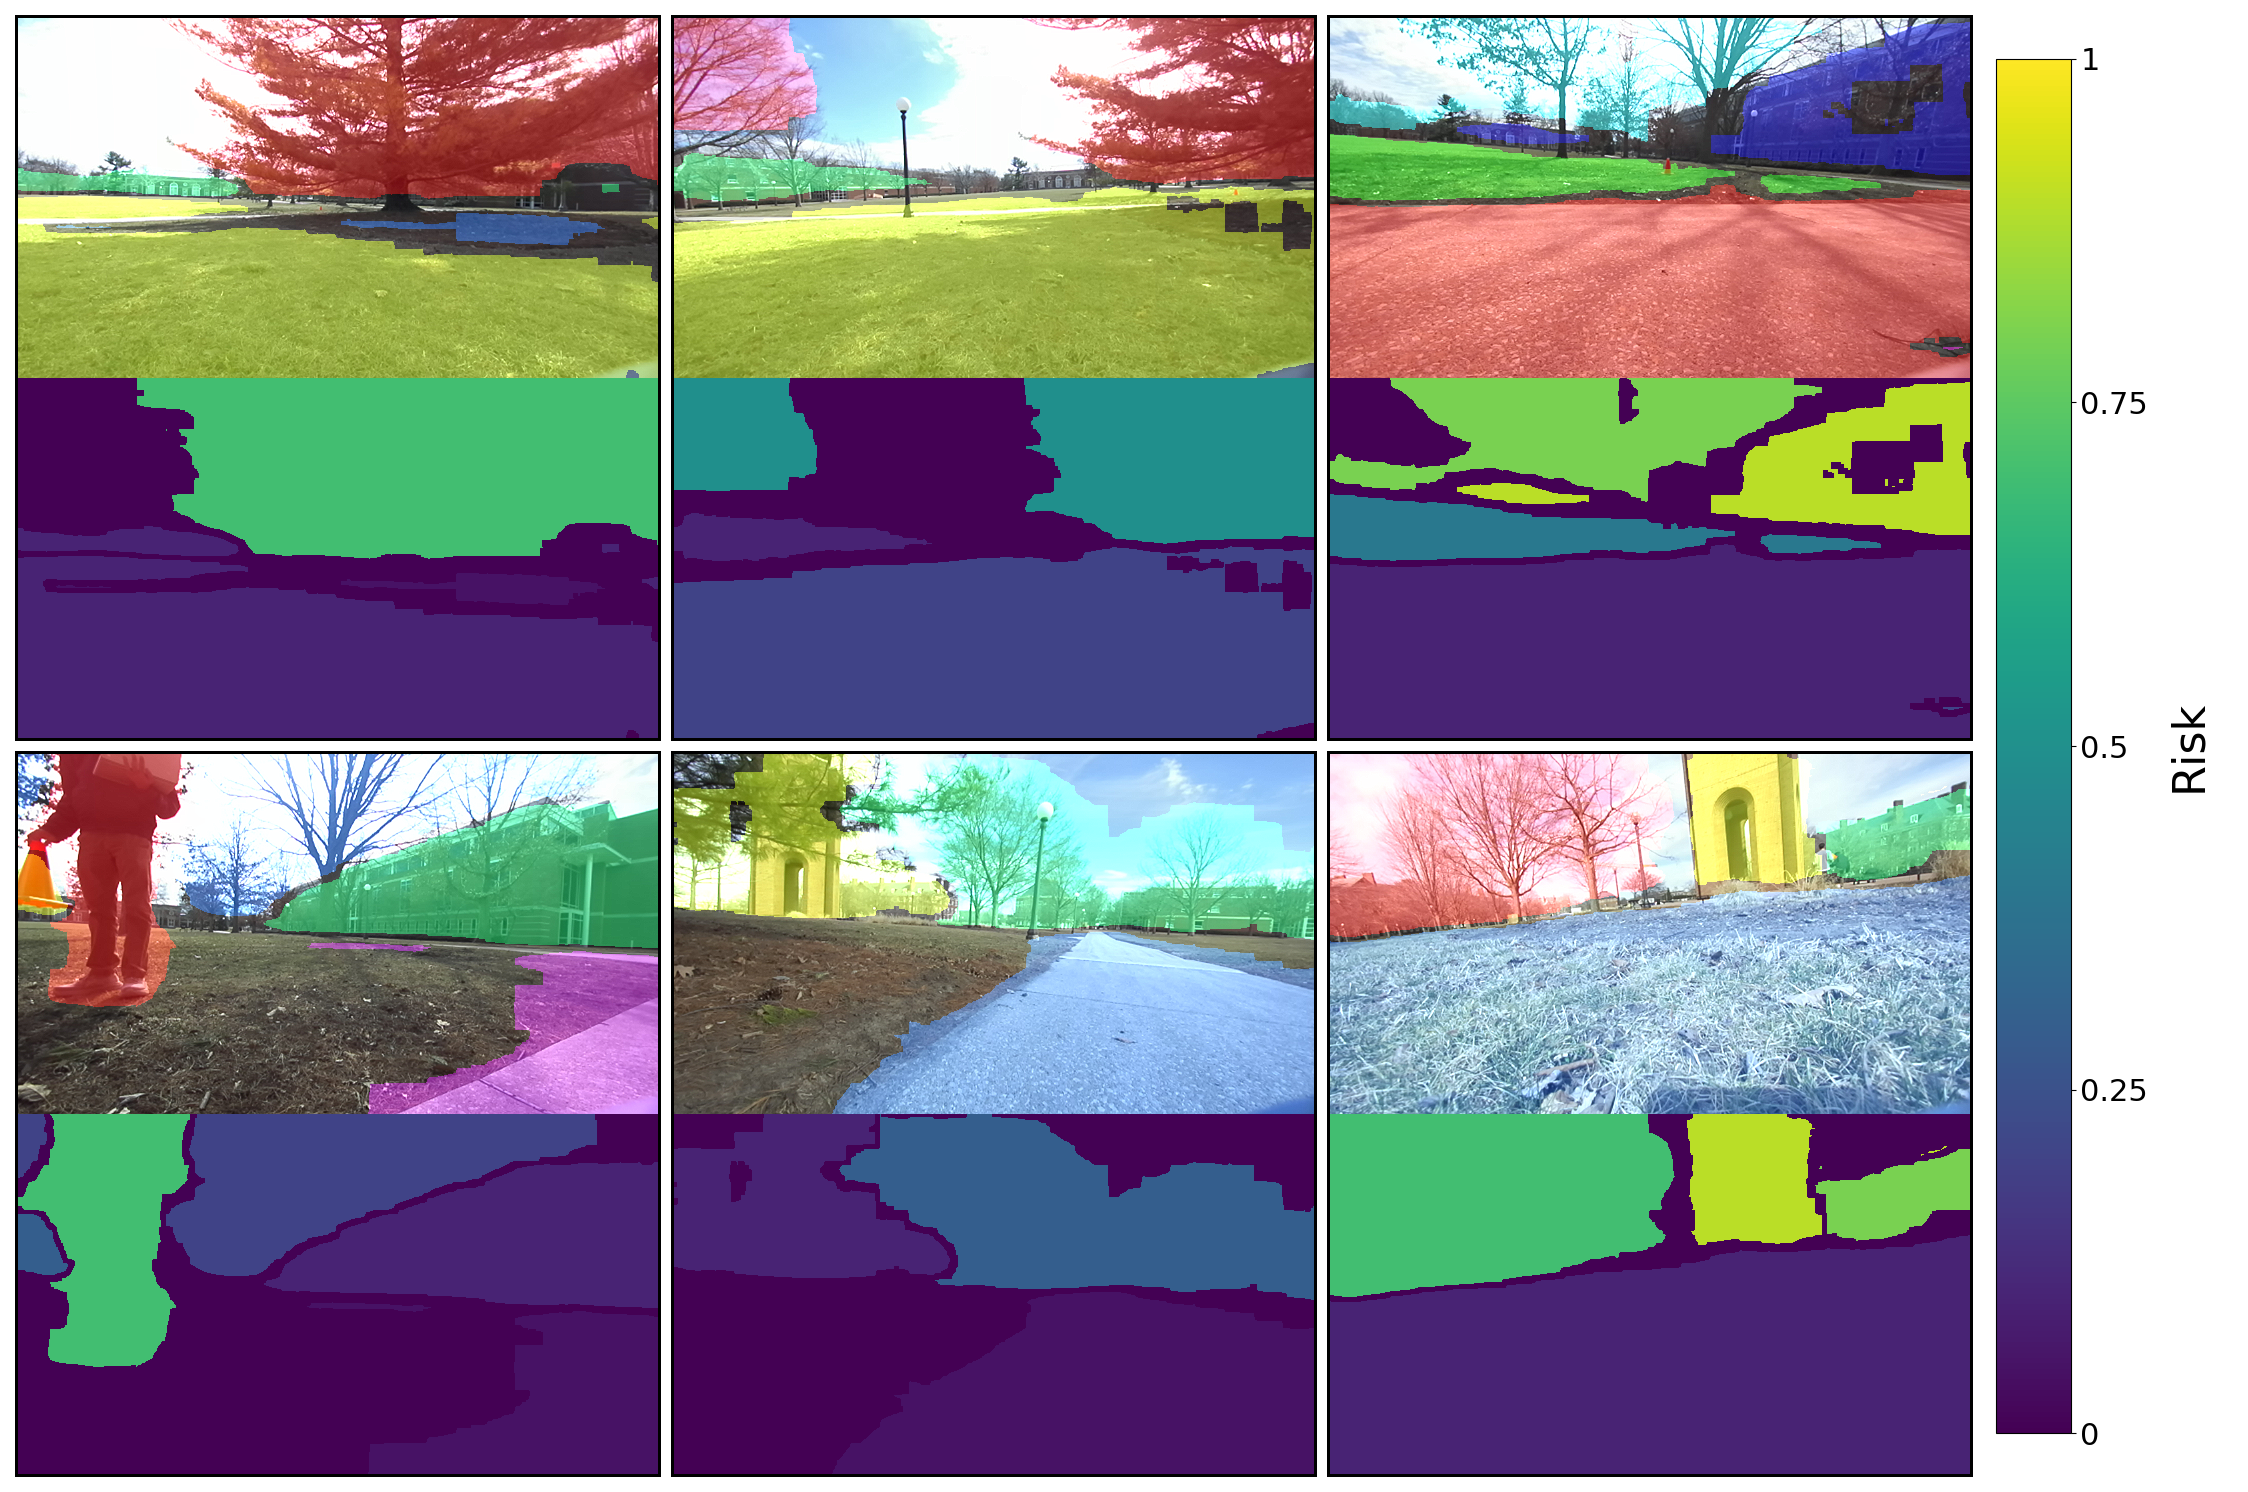
\includegraphics[height=50mm]{catnav_cost.png}

  \takeaway{領域ごとにコストが付く．人や構造物はある程度高いリスクになる．}
\end{frame}

\begin{frame}{結果 ｜ VLM への問い合わせ}
  \source{Potnis et al., arXiv, 2026, Table~II}
  \centering
  {\scriptsize
  \begin{tabular}{lccc}
    \toprule
    & Test 1 & Test 2 & Test 3 \\
    \midrule
    近傍数 $k$ & 1 & 5 & 5 \\
    新規性の閾値 $\gamma$ & 0.55 & 0.1 & 0.55 \\
    シーン問い合わせ & 16 & 125 & 9 \\
    経路選択の呼び出し & 156 & 295 & 157 \\
    VLM 問い合わせ合計 & 172 & 420 & 166 \\
    問合せ (Q/s) & 0.004 & 0.042 & 0.006 \\
    平均遅延 (s) & 3.937 & 17.35 & 3.717 \\
    \bottomrule
  \end{tabular}
  }

  \vspace{0.35em}
  \infocard[orange]{読み方}{%
    \li Test 2（$\gamma=0.1$）は多くの画像を新規と判断し，問い合わせが約 10 倍になる
    \li Test 3（$k=5$，$\gamma=0.55$）は Test 2 に比べ，VLM への問い合わせを 85.7\% 減らす}

  \takeaway{新規性の閾値を調整すると，画像の問い合わせ回数を減らせる．}
\end{frame}

\begin{frame}{結果 ｜ 柔軟な経路選択}
  \source{Potnis et al., arXiv, 2026, Table~III・Fig.~6．各タスク 10 試行}
  \centering
  {\scriptsize\setlength{\tabcolsep}{3.2pt}
  \begin{tabular}{llcccc}
    \toprule
    & & 到達 & 距離 & 衝突 & 行動違反 \\
    \midrule
    \multirow{2}{*}{道の右側} & OmniVLA & 60\% & 2.7\,m & 20\% & 40\% \\
    & CATNAV & 70\% & 2.8\,m & 10\% & 30\% \\
    \multirow{2}{*}{道の中央} & OmniVLA & 50\% & 2.3\,m & -- & 20\% \\
    & CATNAV & 70\% & 2.25\,m & -- & 20\% \\
    \multirow{2}{*}{人が横切る} & OmniVLA & 60\% & 0.4\,m & 20\% & -- \\
    & CATNAV & 70\% & 0.3\,m & 20\% & -- \\
    \multirow{2}{*}{ベンチ} & OmniVLA & 30\% & 0.8\,m & 20\% & -- \\
    & CATNAV & 40\% & 0.7\,m & 30\% & -- \\
    \multirow{2}{*}{床の紙} & OmniVLA & 90\% & 0.1\,m & 0\% & 70\% \\
    & CATNAV & 90\% & 0.1\,m & 0\% & 30\% \\
    \bottomrule
  \end{tabular}
  }

  \vspace{0.12em}
  \centering
  {\scriptsize
  \begin{tabular}{@{}cccc@{}}
    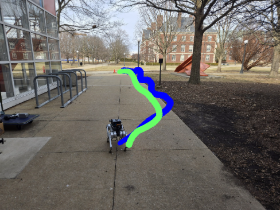
\includegraphics[height=11mm]{catnav_traj_foot.png} &
    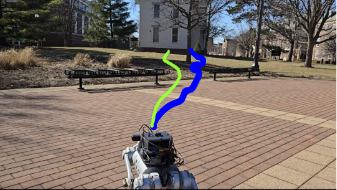
\includegraphics[height=11mm]{catnav_traj_bench.png} &
    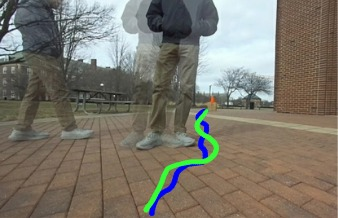
\includegraphics[height=11mm]{catnav_traj_human.png} &
    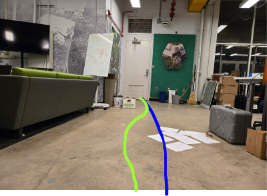
\includegraphics[height=11mm]{catnav_traj_paper.png} \\[-0.15em]
    道 & ベンチ & 人 & 紙
  \end{tabular}
  }

  \takeaway{到達率は平均 68\% 対 58\%．紙をよけるなど，行動違反は 33\% 少ない．}
\end{frame}

\begin{frame}{まとめ ｜ CATNAV}
  \source{Potnis et al., arXiv, 2026}
  \begin{columns}[T,onlytextwidth]
    \begin{column}{0.49\textwidth}
      \infocard[green][46mm]{貢献}{%
        \li タスク学習なしで，意味的リスクをゼロショット推定
        \li 類似シーンの評価を再利用し，問い合わせを 85.7\% 削減
        \li 画像上の複数経路から，理由つきで一本を選ぶ
        \li 好みは，経路選択の指示として入る}
    \end{column}
    \hfill
    \begin{column}{0.49\textwidth}
      \infocard[orange][46mm]{リミテーション}{%
        \li 2D--3D 変換でノイズが出る
        \li 軌道の固定パラメータが数か所ある
        \li CLIP-Seg など，基盤モデルの能力に依存する
        \li 細い障害物は遠方でリスクを過小評価しうる}
    \end{column}
  \end{columns}

  \takeaway{好みはコストの数値と，見た目による経路選択の二段で表現される．}
\end{frame}

% ---------- SEA-Nav ----------

\begin{frame}{SEA-Nav}
  \source{Chen et al., arXiv, 2026}
  \centering
  \begin{tikzpicture}[x=8.6mm, y=8.6mm, font=\scriptsize, box/.style={align=center, minimum height=8mm, text width=20mm, inner sep=1.5pt}]
    \node[font=\scriptsize\bfseries, text=muted] at (0.2,2.15) {通常の Actor-Critic};
    \node[kw, draw=cplaintt, fill=cplain, box] (e1) at (0,0.85) {Environment};
    \node[kwblue, box] (a1) at (3.05,0.85) {Actor};
    \node[kwgreen, box] (c1) at (3.05,-0.55) {Critic};
    \draw[kwarr] (e1) -- (a1);
    \draw[kwarr] (a1.south) -- (c1.north)
      node[midway, right, font=\scriptsize, text=muted] {行動};

    \node[font=\scriptsize\bfseries, text=cbluett] at (7.15,2.15) {SEA-Nav};
    \node[kw, draw=cplaintt, fill=cplain, box] (e2) at (6.9,0.85) {Environment};
    \node[kwblue, box] (a2) at (9.7,0.85) {Actor};
    \node[kworange, box, text width=15mm] (s) at (12.15,0.85) {LSE-CBF};
    \node[kwgreen, box] (c2) at (9.7,-0.7) {Critic};
    \draw[kwarr] (e2) -- (a2);
    \draw[kwarr] (a2) -- (s);
    \draw[kwarr] (s.south) -- (s.south |- c2.east) -- (c2.east)
      node[pos=0.22, right, font=\scriptsize, text=muted] {安全な行動};
  \end{tikzpicture}

  \vspace{0.45em}
  \infocard[blue]{評価の対象}{%
    \li 通常は Actor の生の行動を Critic が見る
    \li SEA-Nav は，CBF で安全範囲へ動かした行動を Critic が評価する}

  \takeaway{安全フィルタは後処理ではなく，方策の一部として誤差が伝わる．}
\end{frame}

\begin{frame}{背景}
  \source{Chen et al., arXiv, 2026}
  \infocard[orange][18mm]{自立ナビゲーション}{%
    \li 密な障害物の中の移動は難しく，安全性を上げる必要がある
    \li 大規模な事前学習で，局所環境の性能は上がってきた}
  \vspace{0.3em}
  \infocard[blue][20mm]{安全ナビと CBF}{%
    \li Actor-Critic の外に CBF を置くと，方策は補正されたことを知らない
    \li 失敗でエピソードが終わると，その直前のデータを学習に使いづらい
    \li 取れる失敗サンプルの母数が少ない}

  \takeaway{フィルタの介入も含めて学び，衝突の前後を効率よくサンプルしたい．}
\end{frame}

\begin{frame}{従来手法}
  \source{Chen et al., arXiv, 2026}
  \begin{columns}[T,onlytextwidth]
    \begin{column}{0.32\textwidth}
      \infocard[plain][30mm]{模倣学習}{%
        \li 行動をまねる
        \li 未知だと失敗しやすい}
    \end{column}
    \hfill
    \begin{column}{0.32\textwidth}
      \infocard[orange][30mm]{深層強化学習}{%
        \li 機動性は出る
        \li 密集すると失敗が多い
        \li 安全制限を掛けにくい}
    \end{column}
    \hfill
    \begin{column}{0.32\textwidth}
      \infocard[blue][30mm]{後処理フィルタ}{%
        \li CBF は Actor の外にある
        \li 方策は補正を知らない
        \li 介入を学習できない}
    \end{column}
  \end{columns}

  \takeaway{サンプル効率と，フィルタ込みの安全制御が同時に欲しい．}
\end{frame}

\begin{frame}{貢献}
  \source{Chen et al., arXiv, 2026}
  \cardbalance
  \infocard[blue][16mm]{貢献 1 ｜ End-to-End LSE-CBF}{%
    \li 安全条件を滑らかにし，学習時とテスト時の不一致をなくす}
  \vspace{0.28em}
  \infocard[orange][16mm]{貢献 2 ｜ 運動学的な正則化}{%
    \li 速度の範囲と変化の滑らかさを損失に入れ，実機へ安全に載せる}
  \vspace{0.28em}
  \infocard[green][16mm]{貢献 3 ｜ ACSI}{%
    \li 衝突前後を巻き戻して学び，サンプル効率のボトルネックを減らす}
  \takeawaybalance{安全層・正則化・衝突の再利用の三つで，短い学習でも走破する．}
\end{frame}

\begin{frame}{モデル構造}
  \source{Chen et al., arXiv, 2026, Fig.~2}
  \centering
  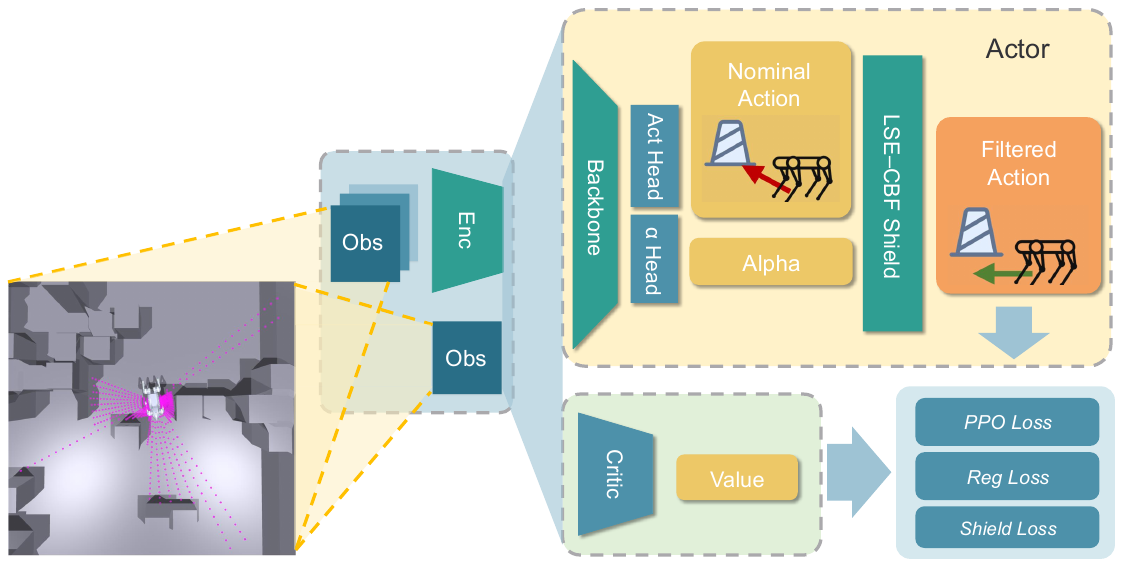
\includegraphics[width=\textwidth,height=42mm,keepaspectratio]{seanav_arch.png}

  \takeaway{Actor は希望速度と $\alpha$ を出し，LSE-CBF を通した速度を損失で学ぶ．}
\end{frame}

\begin{frame}{通常の Actor-Critic との違い}
  \source{Chen et al., arXiv, 2026}
  \cardbalance
  \begin{columns}[T,onlytextwidth]
    \begin{column}{0.49\textwidth}
      \infocard[plain][32mm]{通常}{%
        \li Actor が行動を出す
        \li Critic はそのままの行動を評価する
        \li 安全フィルタの介入は学習に入らない}
    \end{column}
    \hfill
    \begin{column}{0.49\textwidth}
      \infocard[blue][32mm]{SEA-Nav}{%
        \li Actor の行動を LSE-CBF が安全範囲へ動かす
        \li Critic は動かしたあとの行動を評価する
        \li どの指令が悪いか，誤差が伝わる}
    \end{column}
  \end{columns}
  \takeawaybalance{SEA-Nav は CBF で安全範囲の行動を評価する．}
\end{frame}

\begin{frame}{Actor が決める行動}
  \source{Chen et al., arXiv, 2026, Fig.~2}
  \begin{columns}[T,onlytextwidth]
    \begin{column}{0.50\textwidth}
      \infocard[blue][22mm]{入力}{%
        \li 行動履歴 10 フレームの特徴量
        \li 現在の観測
        \lii 41 本のレイで，障害物までの距離}
      \vspace{0.25em}
      \infocard[green][18mm]{出力}{%
        \li 希望する速度指令 $\bar{u}$
        \li CBF の安全制約に関するパラメータ $\alpha$}
    \end{column}
    \hfill
    \begin{column}{0.46\textwidth}
      \centering
      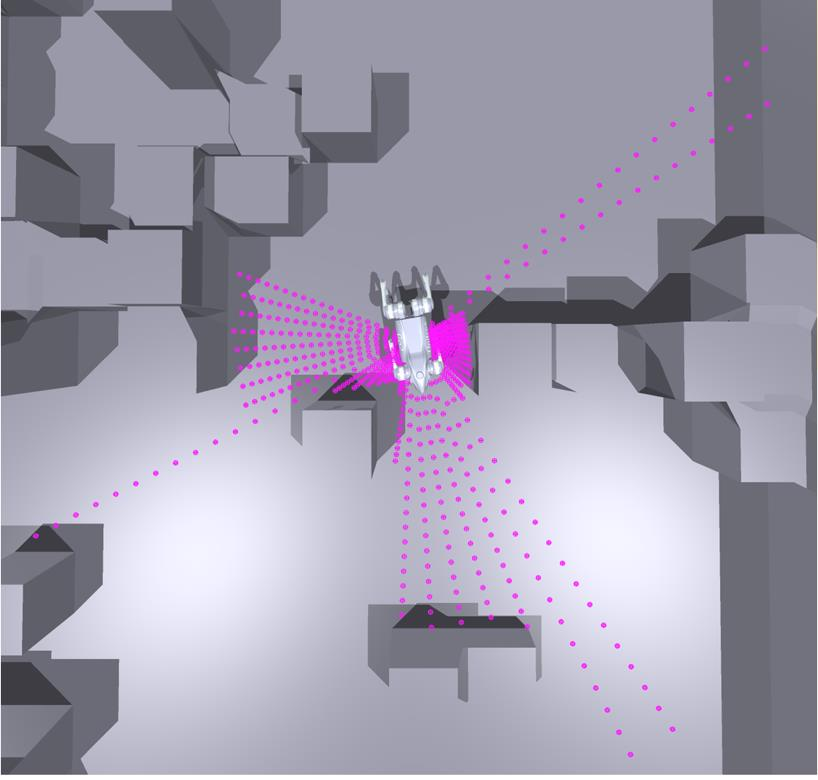
\includegraphics[width=\linewidth,height=46mm,keepaspectratio]{seanav_rays.png}
    \end{column}
  \end{columns}

  \takeaway{方策は速度だけでなく，どれだけ安全側に倒すか $\alpha$ も自分で決める．}
\end{frame}

\begin{frame}{貢献 1 ｜ LSE-CBF}
  \source{Chen et al., arXiv, 2026}
  {\footnotesize\color{body} 各レイの安全条件\hfill
  $h_i(x)=\rho_i-d_{\mathrm{safe}}$}

  \vspace{0.25em}
  \begin{columns}[T,onlytextwidth]
    \begin{column}{0.46\textwidth}
      \infocard[orange][20mm]{通常の CBF}{%
        \li $\displaystyle h(x)=\min_{i\in\{1,\ldots,N\}} h_i(x)$
        \li 最小のレイが入れ替わると不連続
        \li どの指令が悪いか，誤差を流しにくい}
    \end{column}
    \hfill
    \begin{column}{0.52\textwidth}
      \infocard[blue][20mm]{LSE-CBF}{%
        \li $\displaystyle h(x)=-\frac1k\ln\!\Bigl(\sum_{i=1}^{N}\exp(-k\,h_i(x))\Bigr)$
        \li 連続なので，悪い指令へ誤差が伝わる}
    \end{column}
  \end{columns}

  \vspace{0.25em}
  \begin{columns}[T,onlytextwidth]
    \begin{column}{0.38\textwidth}
      \infocard[plain][16mm]{CBF の安全制約}{%
        \li $\dot h(x,u)\ge -\alpha h(x)$}
    \end{column}
    \hfill
    \begin{column}{0.60\textwidth}
      \infocard[green][16mm]{入力を安全な範囲に最小限動かす}{%
        \li $\displaystyle\min_{u_s}\tfrac12\|u_s-\bar{u}(x)\|^2$
        \lii s.t.\ $\langle L_g h(x),u_s\rangle+\alpha h(x)\ge 0$}
    \end{column}
  \end{columns}

  \takeaway{条件を満たす範囲で安全な速度を出し，Critic はその速度を評価する．}
\end{frame}

\begin{frame}{貢献 2 ｜ 損失関数}
  \source{Chen et al., arXiv, 2026}
  {\footnotesize
  \[
    L_{\mathrm{total}}=L_{\mathrm{PPO}}+\lambda_{\mathrm{shield}}L_{\mathrm{shield}}+\lambda_{\mathrm{reg}}L_{\mathrm{reg}}
  \]
  }
  \vspace{-0.7em}
  \infocard[orange]{$L_{\mathrm{shield}}$}{%
    \li CBF のパラメータの損失．過剰介入と過剰抑制を避ける
    \li $L_{\mathrm{shield}}=\|u_{s,t}-\bar{u}_t\|^2+[\alpha_{\min}-\alpha_t]_{+}^{2}$}
  \vspace{0.25em}
  \infocard[green]{$L_{\mathrm{reg}}$　運動学的な正則化}{%
    \li 安全：最大速度を超えない
    \li {\scriptsize $L_{\mathrm{range}}=\sum_{j\in\{x,y,\omega\}}\bigl(u_{s,t}^{j}-\mathrm{clip}(u_{s,t}^{j},u_{j}^{\min},u_{j}^{\max})\bigr)^{2}$}
    \li なめらか：急に方針を変えない
    \li $L_{\mathrm{smooth}}=\lambda_{\pi} D\bigl(\pi_{\theta}(x_t),\pi_{\theta}(\bar{x}_t)\bigr)+\lambda_{V} D\bigl(V_{\phi}(x_t),V_{\phi}(\bar{x}_t)\bigr)$}

  \takeaway{正則化により，実機で安全かつ滑らかな速度指令を出せる．}
\end{frame}

\begin{frame}{貢献 3 ｜ ACSI}
  \source{Chen et al., arXiv, 2026}
  \infocard[blue][14mm]{バッファ}{%
    \li 直近 2 秒，100 ステップを保持し，衝突後には大きなペナルティを与える}
  \vspace{0.22em}
  \begin{columns}[T,onlytextwidth]
    \begin{column}{0.48\textwidth}
      \infocard[orange][20mm]{巻き戻し}{%
        \li $P_{\mathrm{reset}}$ で早期終了し，次のエピソードへ進む
        \li $P_{\mathrm{replay}}$ で 2 秒戻り，回避をやり直す}
    \end{column}
    \hfill
    \begin{column}{0.50\textwidth}
      \infocard[green][20mm]{リセット率}{%
        \li ゴール率に合わせて動的に変える
        \li $P_{\mathrm{reset}}=P_{\min}+(P_{\max}-P_{\min})\cdot\mathrm{clip}(L_{\mathrm{goal}}/1.5,\,0,\,1)$}
    \end{column}
  \end{columns}

  \takeaway{衝突した履歴を効率よく引くので，危険な局所を重点的に学べる．}
\end{frame}

\begin{frame}{結果 ｜ シミュレーション}
  \source{Chen et al., arXiv, 2026, Table~I．RTX 4090 で 2000 iter，約 1 時間}
  {\scriptsize\color{body} 10\,m 四方．密度は Easy / Medium / Hard．数値は成功率 SR（\%）．}

  \vspace{0.3em}
  \centering
  {\scriptsize
  \begin{tabular}{lccc}
    \toprule
    & Easy & Medium & Hard \\
    \midrule
    SEA-Nav & \textbf{100.0} & \textbf{97.0} & \textbf{90.0} \\
    ACSI なし & 100.0 & 93.0 & 83.0 \\
    Shield なし & 97.7 & 90.0 & 74.3 \\
    $L_{\mathrm{reg}}$ なし & 96.3 & 82.3 & 57.0 \\
    \bottomrule
  \end{tabular}
  }

  \vspace{0.35em}
  \infocard[green]{Hard での衝突率}{%
    \li SEA-Nav は 5\%．ACSI なしは 8\%，Shield なしは 12\%，$L_{\mathrm{reg}}$ なしは 18\%
    \li 三つの方法を入れると，難しい環境での走破がまとめて上がる}

  \takeaway{寄与は Easy では小さく，障害物が密な Hard で差が開く．}
\end{frame}

\begin{frame}{結果 ｜ 実機}
  \source{Chen et al., arXiv, 2026, Table~II・Fig.~5．Unitree Go2}
  \centering
  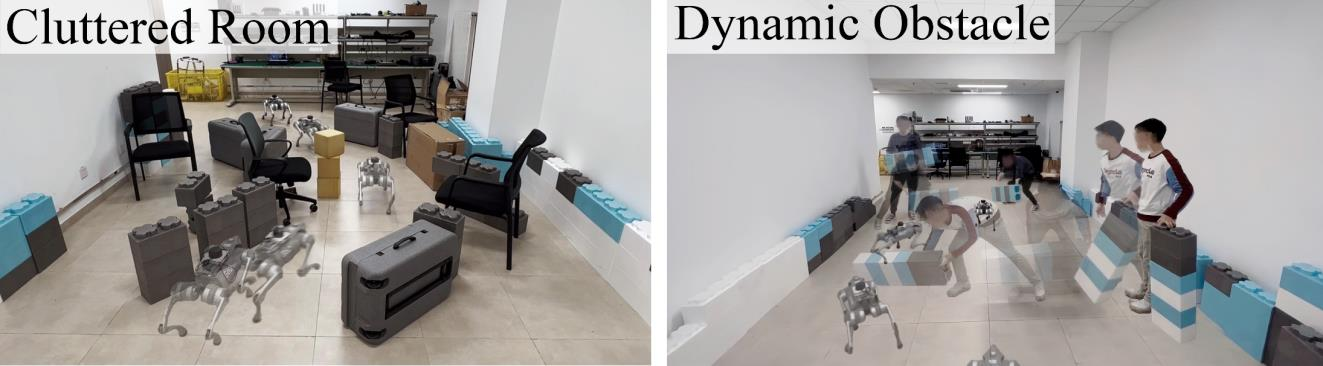
\includegraphics[width=0.49\textwidth,height=20mm,keepaspectratio]{seanav_real_ab.png}\hfill
  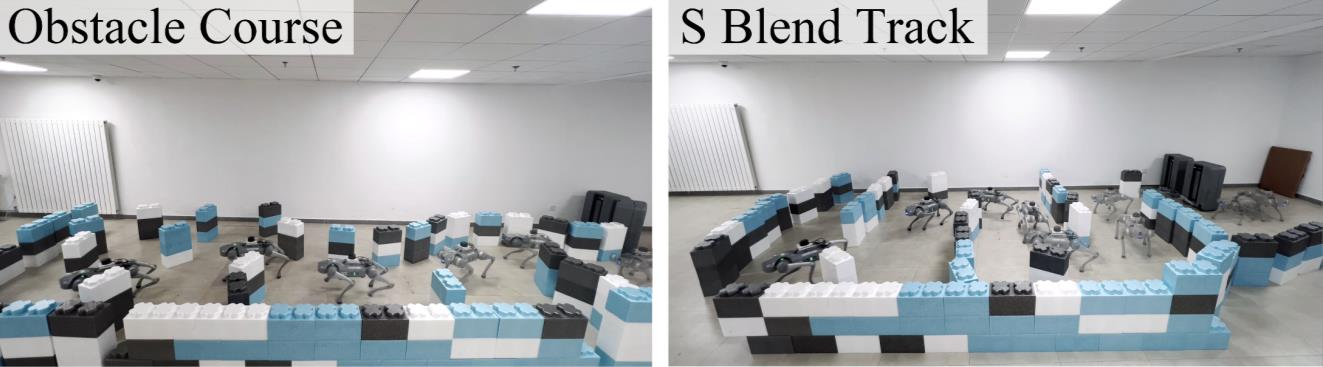
\includegraphics[width=0.49\textwidth,height=20mm,keepaspectratio]{seanav_real_cd.png}

  \vspace{0.25em}
  {\scriptsize\color{body}
  SEA-Nav は学習した歩行モデル，SEA-Nav-b は Unitree 公式の歩行モデル．
  SR は成功率（\%），AS は平均速度（m/s）．}

  \vspace{0.15em}
  \centering
  {\scriptsize\setlength{\tabcolsep}{3pt}
  \begin{tabular}{lcccccccc}
    \toprule
    & \multicolumn{2}{c}{密集した部屋} & \multicolumn{2}{c}{動的障害物} & \multicolumn{2}{c}{障害物コース} & \multicolumn{2}{c}{S 字} \\
    \cmidrule(lr){2-3}\cmidrule(lr){4-5}\cmidrule(lr){6-7}\cmidrule(lr){8-9}
    & SR & AS & SR & AS & SR & AS & SR & AS \\
    \midrule
    SEA-Nav & 100 & 1.6 & 90 & 1.5 & 100 & 1.2 & 100 & 1.4 \\
    SEA-Nav-b & 100 & 0.9 & 100 & 0.8 & 90 & 0.7 & 100 & 0.5 \\
    SLAM & 100 & 0.5 & 80 & 0.4 & 100 & 0.4 & 80 & 0.3 \\
    \bottomrule
  \end{tabular}
  }

  \takeaway{4 環境の多くで SEA-Nav の成功率が高く，公式モデルや SLAM より速い．}
\end{frame}

\begin{frame}{まとめ ｜ SEA-Nav}
  \source{Chen et al., arXiv, 2026}
  \begin{columns}[T,onlytextwidth]
    \begin{column}{0.49\textwidth}
      \infocard[blue][42mm]{貢献}{%
        \li LSE-CBF を方策の中に通し，学習と実行の安全層を一致させる
        \li 運動学の正則化で，実機に出せる速度にする
        \li ACSI で衝突前後を再利用する
        \li Hard で成功率 90\%，約 1 時間の学習}
    \end{column}
    \hfill
    \begin{column}{0.49\textwidth}
      \infocard[orange][42mm]{リミテーション}{%
        \li 平らな路面を想定している
        \li 坂や段差は対象外
        \li 単純な局所解は抜けられる
        \li 複雑な行き止まりや迷路は未対応}
    \end{column}
  \end{columns}

  \takeaway{安全は，速度指令を通す微分可能な制約としてプランナに入る．}
\end{frame}

\begin{frame}{まとめ ｜ 2本のサーベイ}
  \cardbalance
  \begin{columns}[T,onlytextwidth]
    \begin{column}{0.49\textwidth}
      \infocard[green][48mm]{CATNAV ｜ 好み}{%
        \li VLM が意味的なリスクをゼロショットで付ける
        \li 似た画像はキャッシュし，問い合わせを減らす
        \li 複数経路を見て，指示に合う一本を選ぶ
        \li 歩き方の好みは，経路選択の理由として入る}
    \end{column}
    \hfill
    \begin{column}{0.49\textwidth}
      \infocard[blue][48mm]{SEA-Nav ｜ 安全}{%
        \li レイの距離から，安全な速度指令を直接学ぶ
        \li CBF は後処理ではなく，評価と損失に入る
        \li 衝突の巻き戻しで，密集環境を短時間で学ぶ
        \li 安全保障は，速度の制約として入る}
    \end{column}
  \end{columns}
  \takeawaybalance{好みは経路の選択，安全は速度の制約．局所プランナではこの二つを重ねたい．}
\end{frame}

\end{document}
